\section{Buck-converter\label{B-C}}

The task of a buck converter is to be changing the input voltage to a lower output voltage. The components, which are needed, are a DC-source for input voltage, a switch contained of a diode and a MOSFET, an inductor, a capacitor and a resistor for the load. The equivalent diagram in figure 1.1 illustrated a buck-converter with an ideal switch.  

\begin{figure}[htbp]
	\begin{center}
		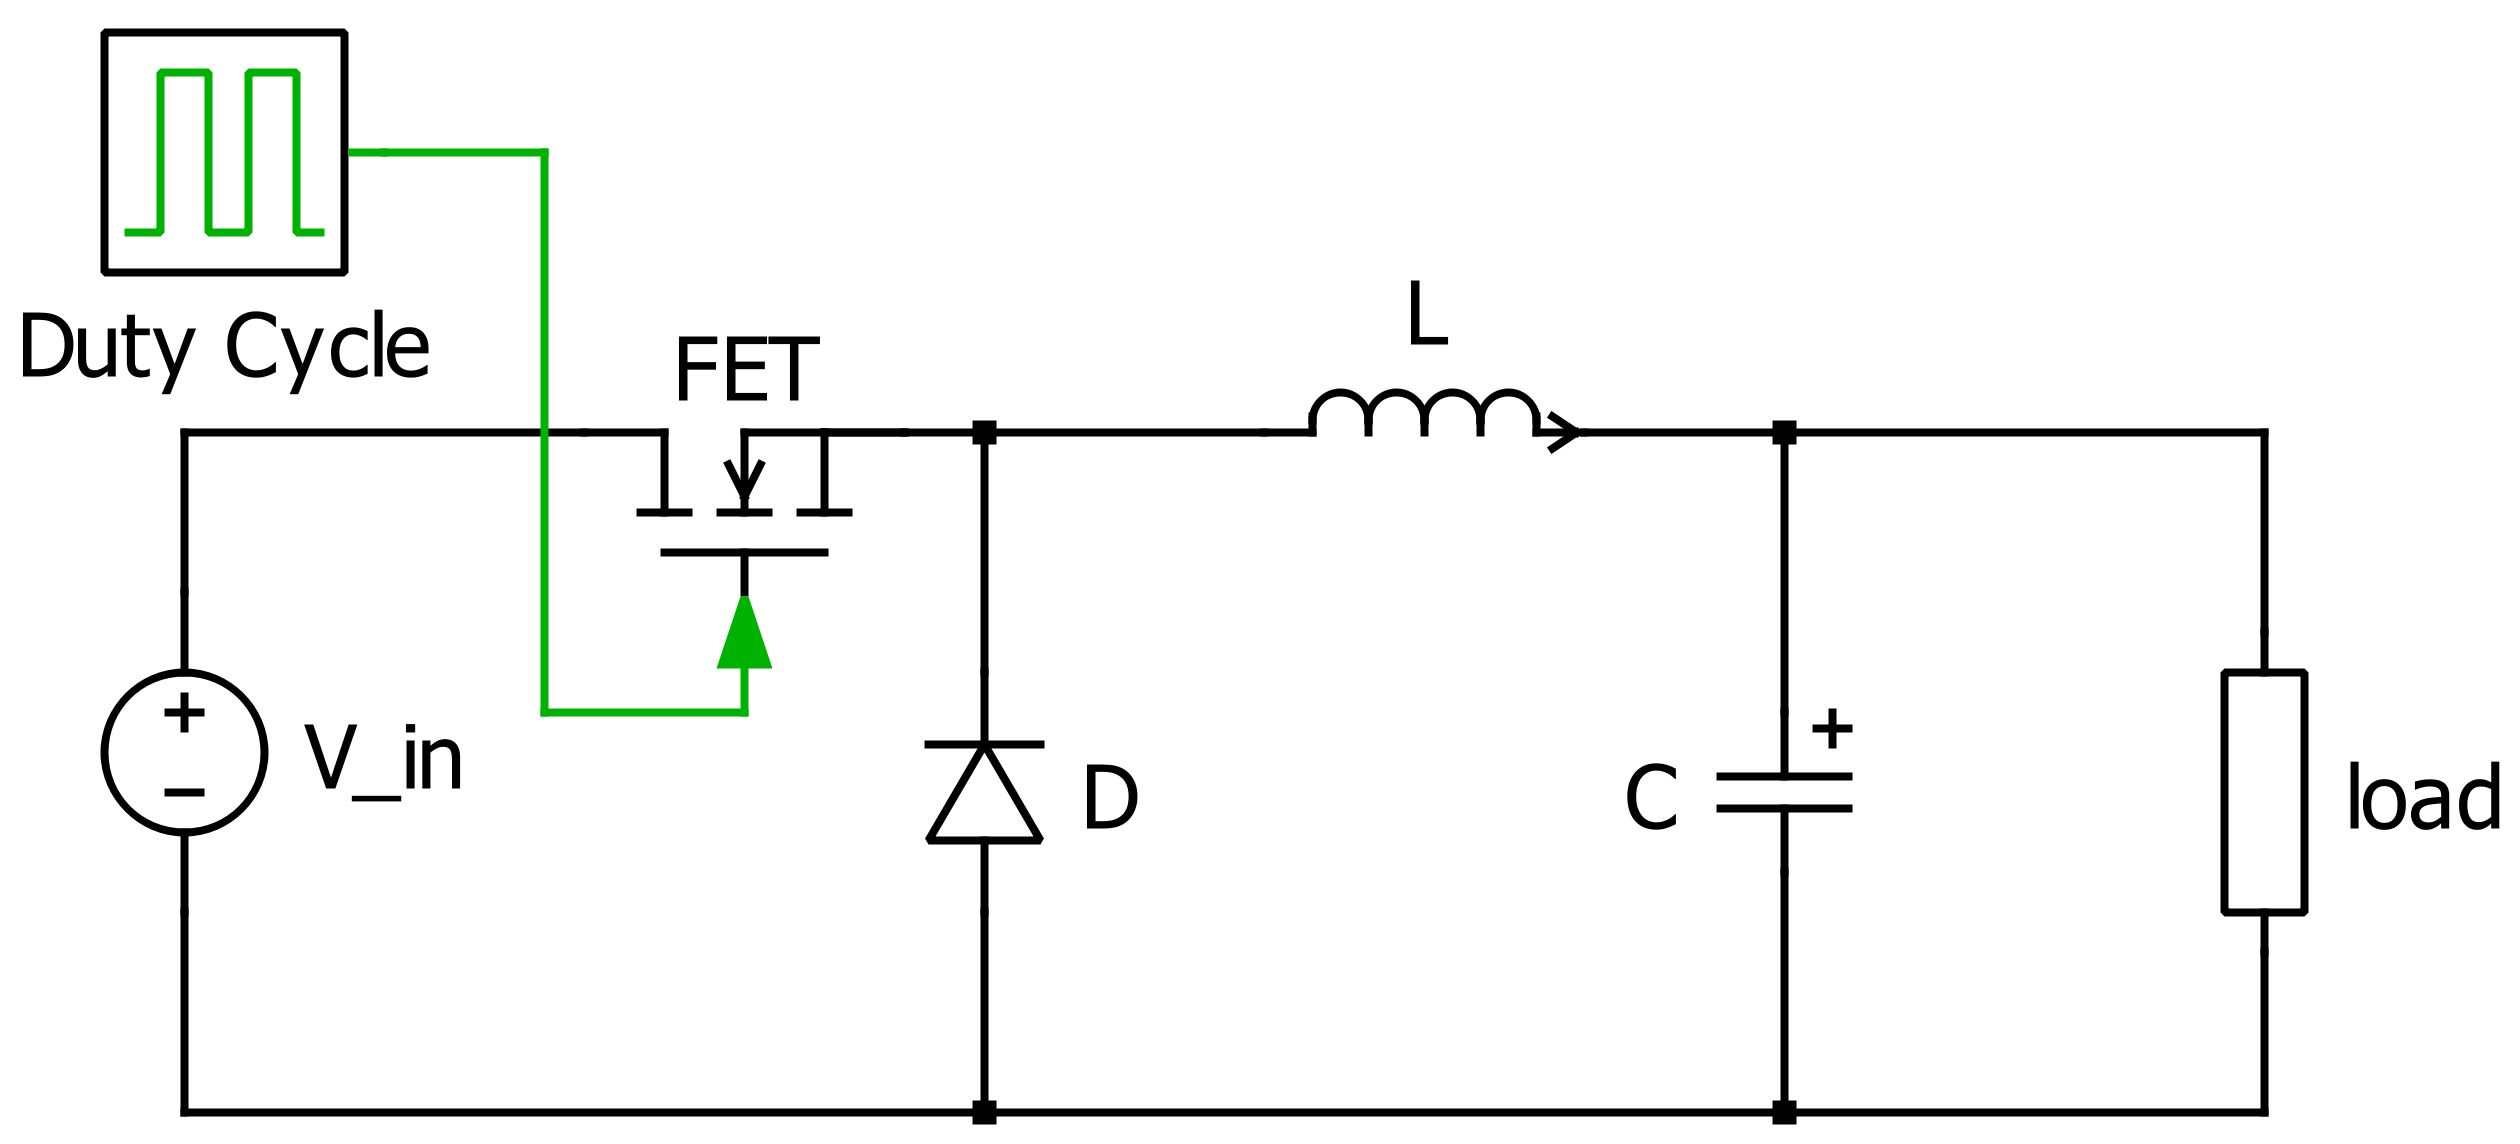
\includegraphics[width=0.7\textwidth]{../Pictures/Buck-converter}
		\caption{Buck-converter.}
		\label{Buck-converter}
	\end{center}	
\end{figure}

A buck-converter perform in two operating modes. In both operating modes have been approach that the converter is in steady state and the average of a value is constant. Therefore, we can assume a DC-voltage at the load. At the case, that the MOSFET conducts current (position 1), the diode will be gesperrt. During the switch is in position 1 the voltage dropes at the inductor and you can measure a lower voltage at the load. Furthermore, the capacitor is charging voltage and the inductor is stored current. For the position 2 the inductor works as a current source and feeds the closed circuit with current. The capacitor enstored is energy from the electrical field.
The advantage for using a buck converter is that the structure is very simple and you need one power switch. The size for the component is small and the cost for this are low. Furthermore, the buck converter has a high effiency over 90 %.

So we come to the disadvantgages eines buck converters. The transient response is slow for changes. The input has got a filter. Thus, could a buck converter no signal, where you need a unfilter signal,can used.
